\documentclass[12pt, fleqn]{article}

\usepackage{amsmath}
\usepackage{amssymb}
\usepackage{amsthm}
\usepackage{mathtools}
\usepackage{hyperref}
\usepackage{ulem}
\usepackage{enumitem}
\usepackage[left=0.75in, right=0.75in, bottom=0.75in, top=1.0in]{geometry}
\usepackage{floatrow}
\usepackage{graphicx}
\usepackage[export]{adjustbox}
\usepackage{sectsty}
\sectionfont{\centering}

\usepackage[dvipsnames]{xcolor}

\usepackage[perpage]{footmisc}

\usepackage{fancyhdr}
\pagestyle{fancy}
\fancyhf{}
\lhead{190100044}
\rhead{CS 252: Lab 4}
\renewcommand{\footrulewidth}{1.0pt}
\cfoot{Page \thepage}

\setlength{\parindent}{0em}

\title{\vspace{-4em}CS 252: Lab 4}
\author{Devansh Jain, 190100044}
\date{\today}

\begin{document}

% \pagenumbering{gobble}
\maketitle
\tableofcontents
\thispagestyle{empty}
\setcounter{page}{0}


\newpage 
\section*{Exercise 2}
\addcontentsline{toc}{section}{Exercise 2}
\setcounter{equation}{0}

\begin{enumerate}
    \item For the given data link, the maximum throughput the ftp flow can achieve is 7739.2 Kbps for Flow 1 and 342.326 Kbps for Flow 2. (Total is 8081.526 Kbps)
    \item Considering RTT as (approx) 20 ms (Twice of delay), theoretically window size which achieved 7739.2 Kbps as throughput is 19348 bytes.
    \item Experimentally, minimum window size at which this throughput was obtained is 19300 bytes.
    \item The maximum achieved throughput is slightly less than the raw data rate of the link ($7739.2 < 8192$) as can be expected, considering the delay incurred and queuing.
    \item For delay = 5 ms, Maximum throughput is (7762.56 Kbps, 343.362 Kbps) at minimum window size of 10800 bytes. \\
    For delay = 10 ms, Maximum throughput is (7739.2 Kbps, 342.326 Kbps) at minimum window size of 19300 bytes. \\
    For delay = 20 ms, Maximum throughput is (7692.48 Kbps, 340.248 Kbps) at minimum window size of 37600 bytes. \\
    Maximum throughput is reduces slightly as we increase the delay (as expected), and the minimum window size increases almost proportionally as we increase the delay. (Theoretical window size also increases almost proportionally as it is dependent on delay) \\
\end{enumerate}


\newpage 
\section*{Exercise 3}
\addcontentsline{toc}{section}{Exercise 3}
\setcounter{equation}{0}

\begin{enumerate}
    \item For \texttt{CBRdataRate = "448Kbps"}, observed Throughput is 461.296 Kbps. \\
    For \texttt{CBRdataRate = "896Kbps"}, observed Throughput is 921.748 Kbps.\\
    For \texttt{CBRdataRate = "1344Kbps"}, observed Throughput is 1382.2 Kbps.
    \item Maximum throughput achieved is 7768.12 Kbps achieved at minimum \texttt{CBRdataRate} of 7560 Kbps.
    \item The maximum achieved throughput is less than the raw data rate of the link ($7768.12 < 8192$) as can be expected, considering the delay incurred and queuing.
\end{enumerate}

\newpage
\section*{Appendix}
\addcontentsline{toc}{section}{Appendix}
\setcounter{equation}{0}

\begin{figure}[H]
    \centering
    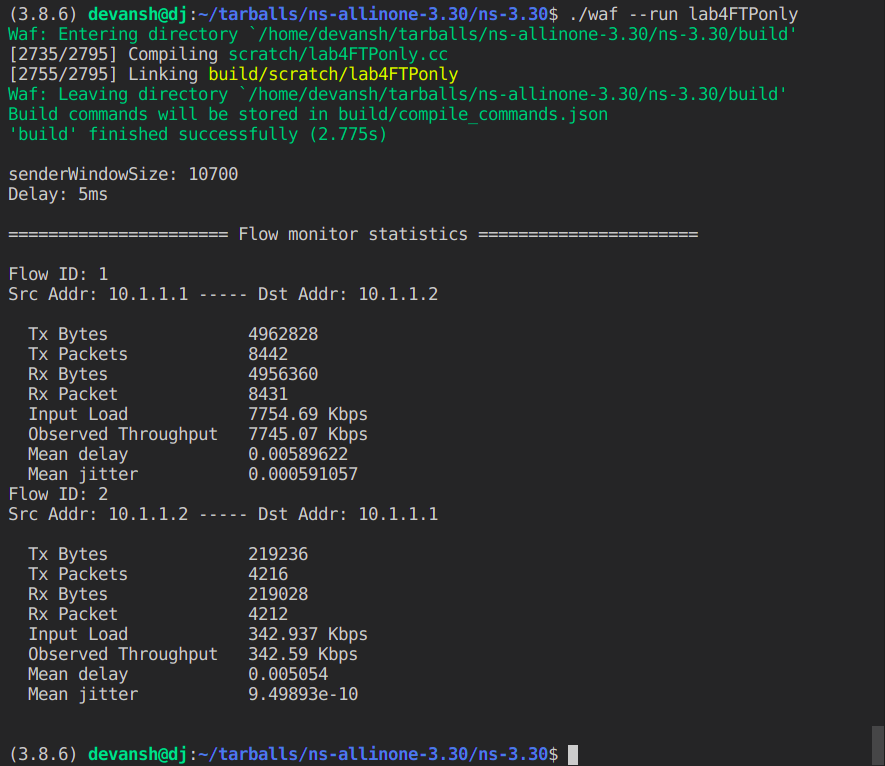
\includegraphics[width=0.6\textwidth]{2_05_10700.png}
    \caption{TCP: Delay 2ms, Window Size 10700 bytes}
\end{figure}
 \begin{figure}[H]
    \centering
    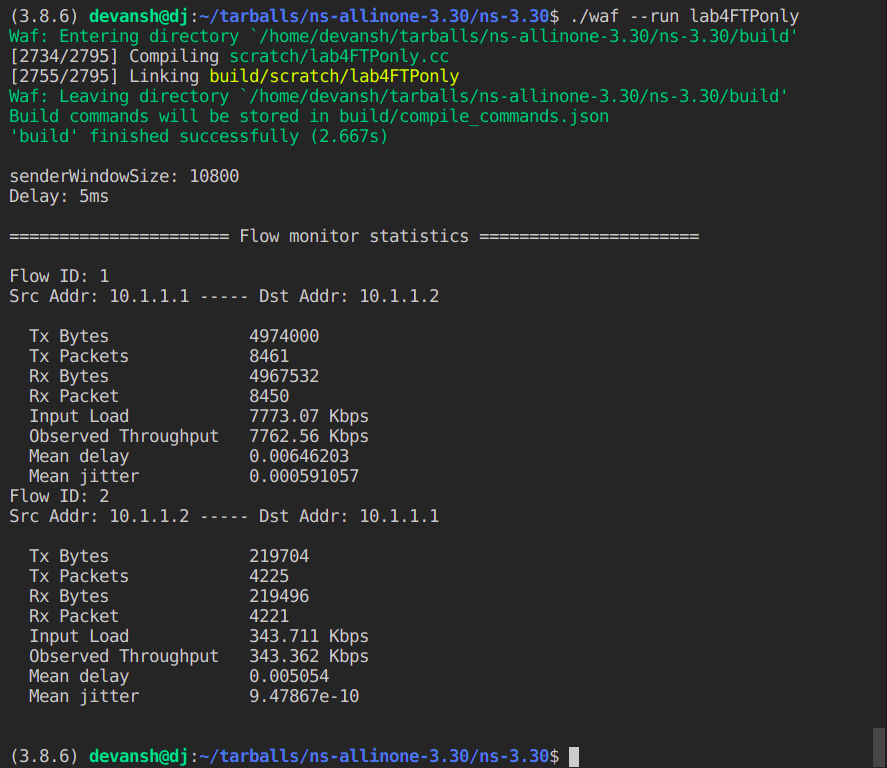
\includegraphics[width=0.6\textwidth]{2_05_10800.png}
    \caption{TCP: Delay 2ms, Window Size 10800 bytes}
\end{figure}
\begin{figure}[H]
    \centering
    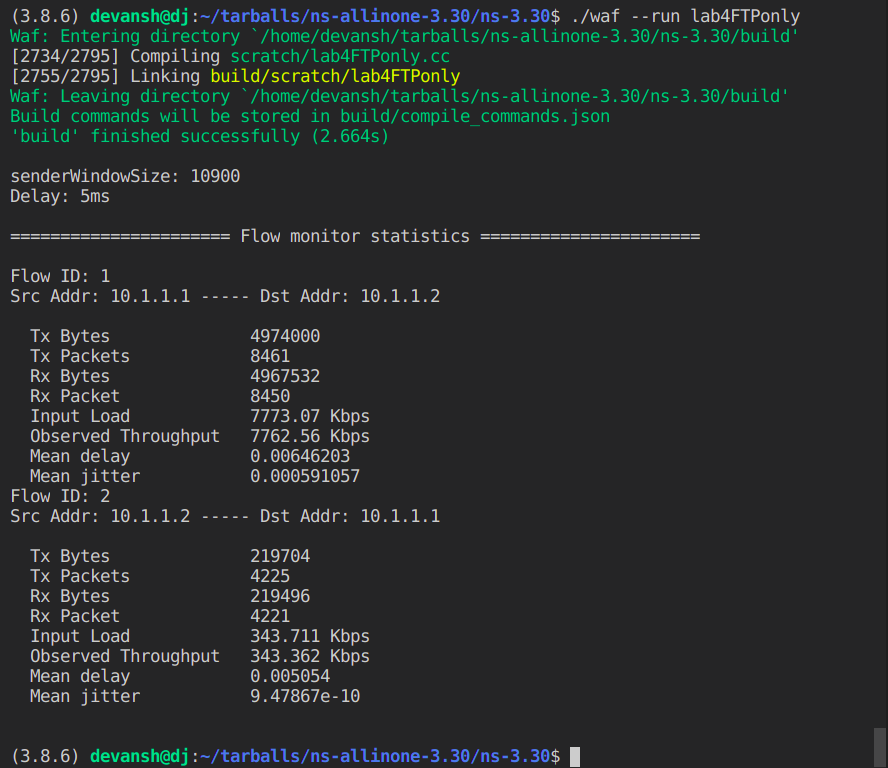
\includegraphics[width=0.6\textwidth]{2_05_10900.png}
        \caption{TCP: Delay 2ms, Window Size 10900 bytes}
\end{figure}
\begin{figure}[H]
    \centering
    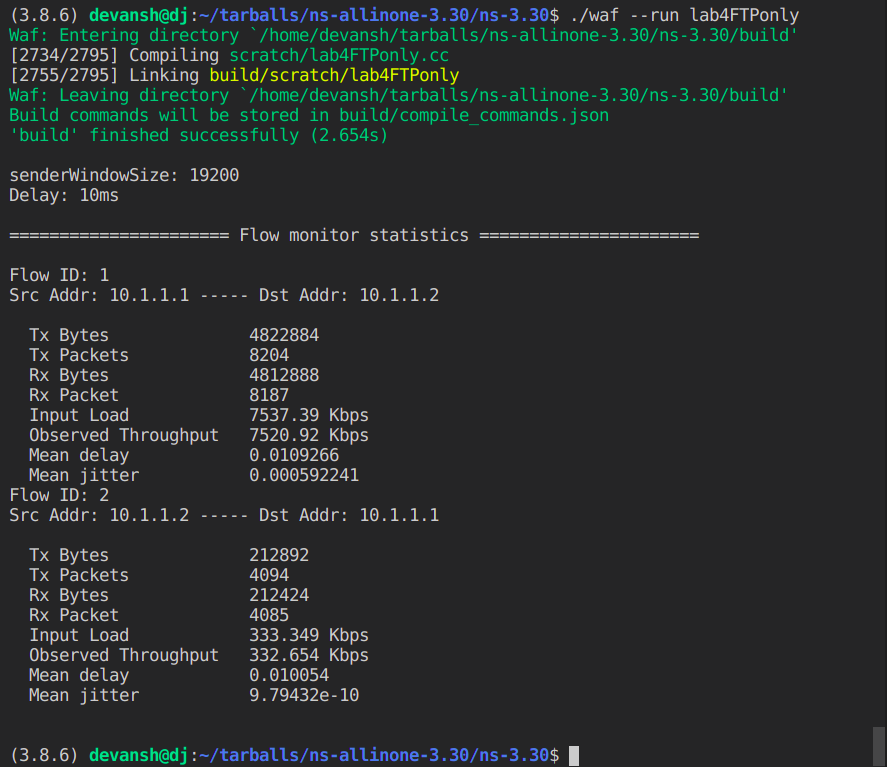
\includegraphics[width=0.6\textwidth]{2_10_19200.png}
    \caption{TCP: Delay 10ms, Window Size 19200 bytes}
\end{figure}
\begin{figure}[H]
    \centering
    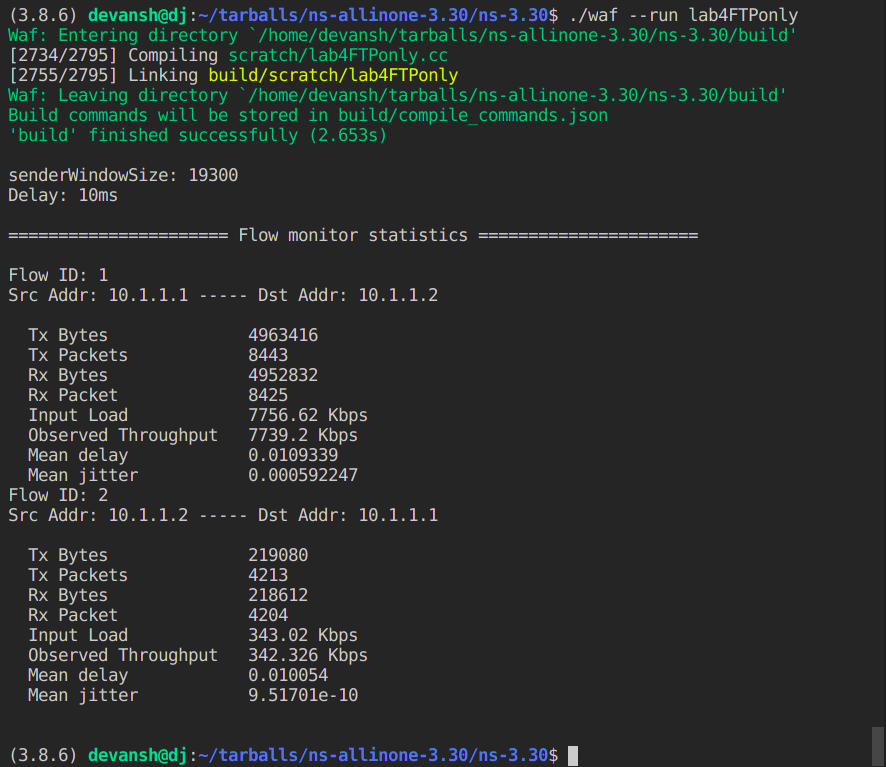
\includegraphics[width=0.6\textwidth]{2_10_19300.png}
    \caption{TCP: Delay 10ms, Window Size 19300 bytes}
\end{figure}
\begin{figure}[H]
    \centering
    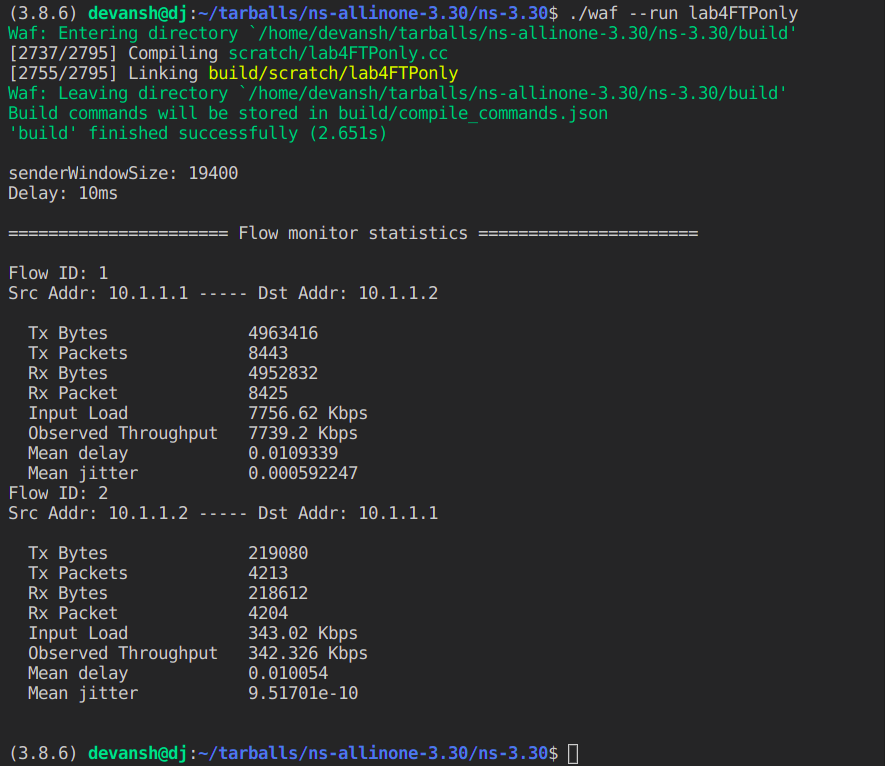
\includegraphics[width=0.6\textwidth]{2_10_19400.png}
    \caption{TCP: Delay 10ms, Window Size 19400 bytes}
\end{figure}
\begin{figure}[H]
    \centering
    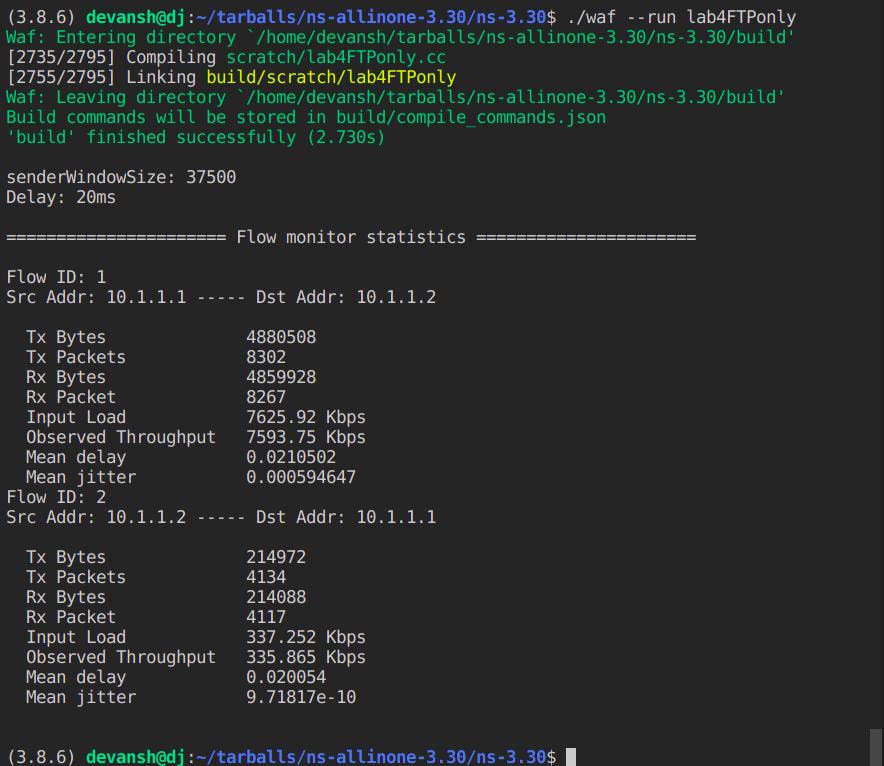
\includegraphics[width=0.6\textwidth]{2_20_37500.png}
    \caption{TCP: Delay 20ms, Window Size 37500 bytes}
\end{figure}
\begin{figure}[H]
    \centering
    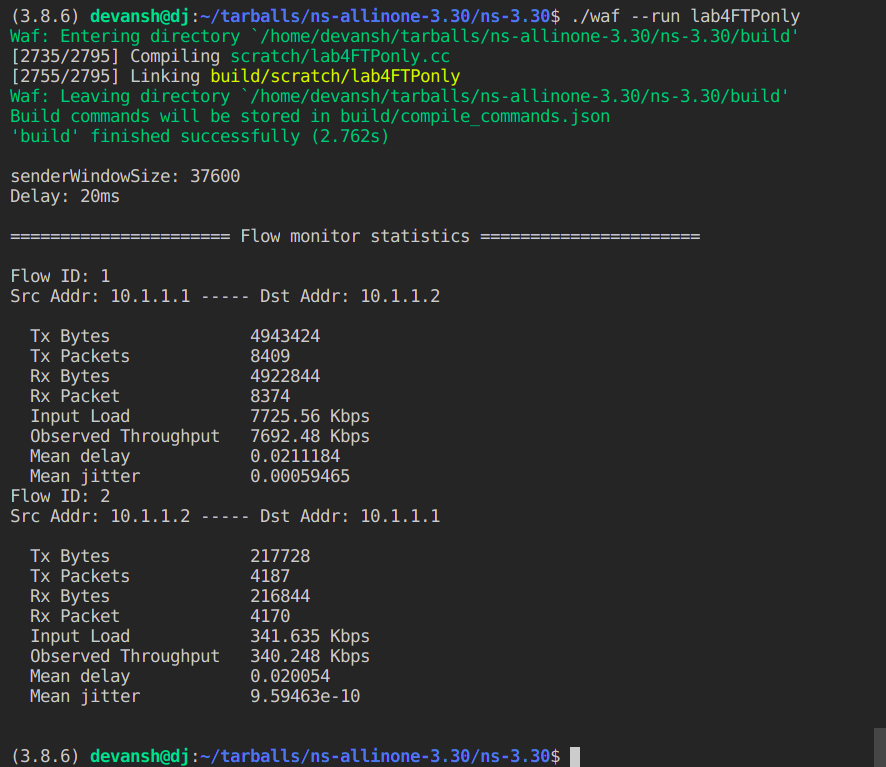
\includegraphics[width=0.6\textwidth]{2_20_37600.png}
    \caption{TCP: Delay 20ms, Window Size 37600 bytes}
\end{figure}
\begin{figure}[H]
    \centering
    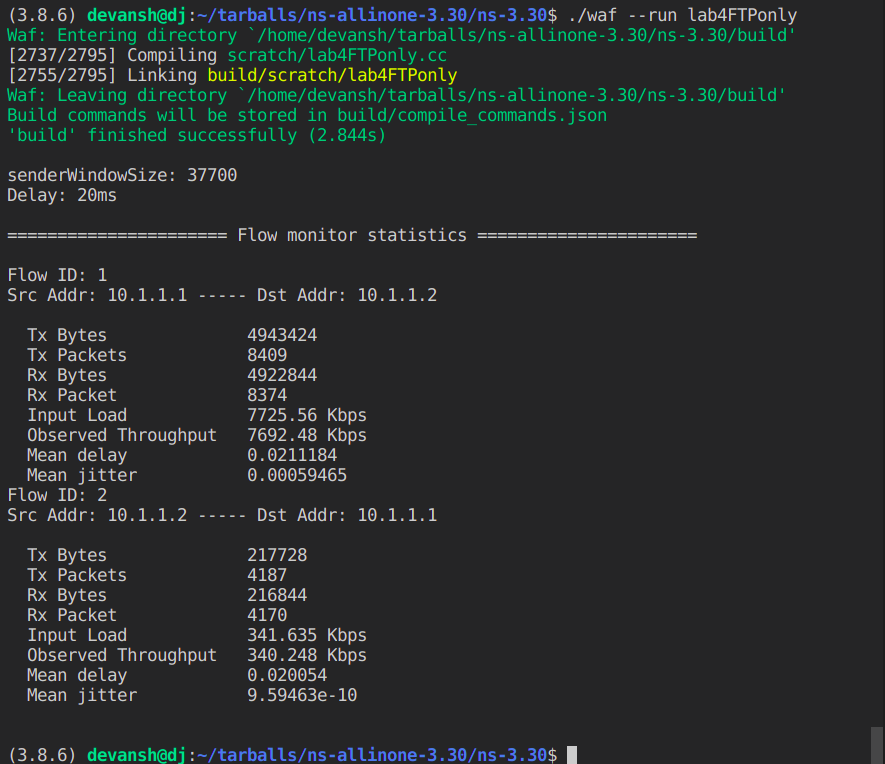
\includegraphics[width=0.6\textwidth]{2_20_37700.png}
    \caption{TCP: Delay 20ms, Window Size 37700 bytes}
\end{figure}
\begin{figure}[H]
    \centering
    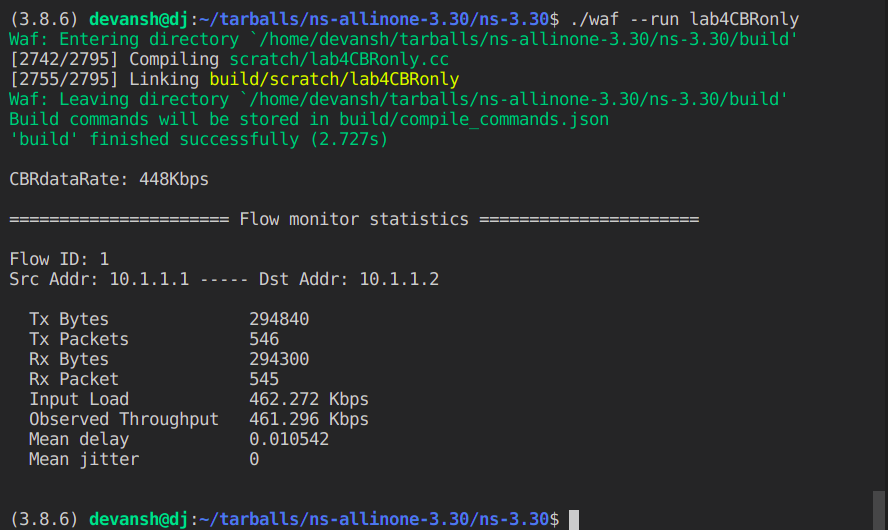
\includegraphics[width=0.6\textwidth]{3_448.png}
    \caption{UDP: CBRdataRate 448 Kbps}
\end{figure}
\begin{figure}[H]
    \centering
    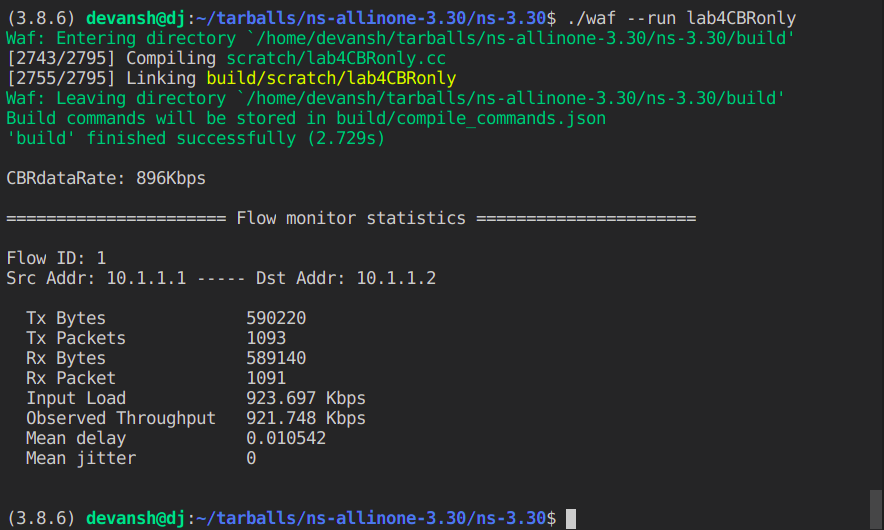
\includegraphics[width=0.6\textwidth]{3_896.png}
    \caption{UDP: CBRdataRate 896 Kbps}
\end{figure}
\begin{figure}[H]
    \centering
    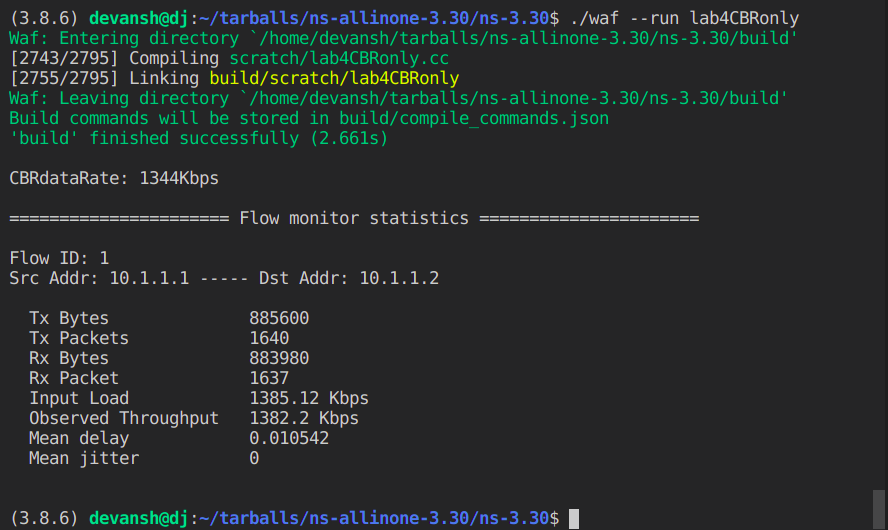
\includegraphics[width=0.6\textwidth]{3_1488.png}
    \caption{UDP: CBRdataRate 1344 Kbps}
\end{figure}
\begin{figure}[H]
    \centering
    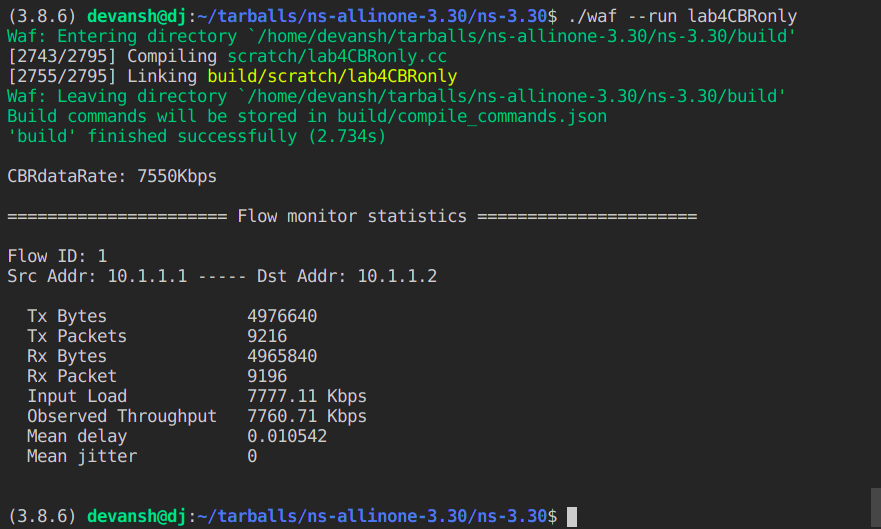
\includegraphics[width=0.6\textwidth]{3_7550.png}
    \caption{UDP: CBRdataRate 7550 Kbps}
\end{figure}
\begin{figure}[H]
    \centering
    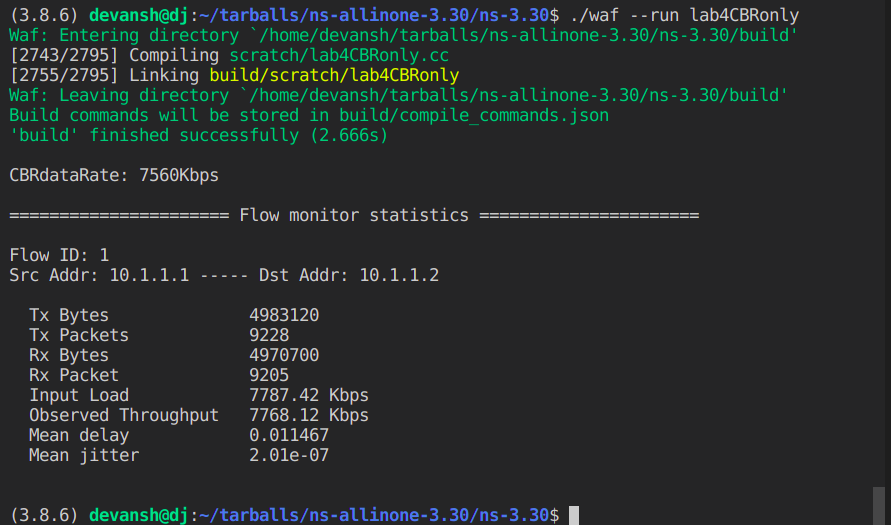
\includegraphics[width=0.6\textwidth]{3_7560.png}
    \caption{UDP: CBRdataRate 7560 Kbps}
\end{figure}
\begin{figure}[H]
    \centering
    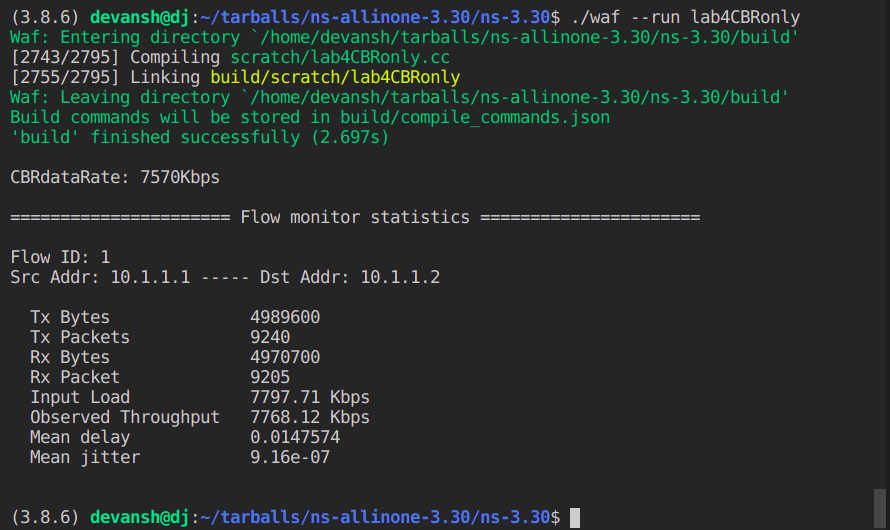
\includegraphics[width=0.6\textwidth]{3_7570.png}
    \caption{UDP: CBRdataRate 7570 Kbps}
\end{figure}

\end{document}
